\documentclass[10pt,twocolumn]{article}          % LaTeX 2e 
\usepackage{latex8}                              % LaTeX 2e 
\usepackage{times}                               % LaTeX 2e 
\usepackage{cite}
\usepackage{graphicx}
\usepackage{amssymb,amsmath,amsthm}
\usepackage{algorithm,algorithmic}
%\usepackage{wasysym}
\usepackage{url}
\usepackage{subfigure}

\newcommand{\domain}[1]{\mathbb{#1}}
\renewcommand{\algorithmiccomment}[1]{ /* #1 */}
\newtheorem{theorem}{Theorem}

%------------------------------------------------------------------------- 
% take the % away on next line to produce the final camera-ready version 
%\pagestyle{empty}

%------------------------------------------------------------------------- 
\begin{document}

\title{SPCVX: Convex Fitting Using B-Splines and Disciplined Convex Programming}

\author{First Author\\
Institution\\
First line of institution address\\ Second line of institution address\\ 
FirstAuthor@institution.com\\
% For a paper whose authors are all at the same institution, 
% omit the following lines up until the closing ``}''.
% Additional authors and addresses can be added with ``\and'', 
% just like the second author.
\and
Second Author\\
Institution2\\
First line of institution2 address\\ Second line of institution2 address\\ 
SecondAuthor@institution2.com\\
}

\maketitle
\thispagestyle{empty}

\begin{abstract}
\end{abstract}

%------------------------------------------------------------------------- 

\Section{Introduction}
\label{sec:intro}
The motivation of convex fitting is as follows. In recent years, the
technique of using geometric programming is emerging with applications such
as analog circuit sizing. However, very often a constraint function
may be too complicated to be written in a posynomial form by hand
analysis. Thus people take another approach that runs many simulations
using an existing circuit simulator such as SPICE, and then perform data
fitting technique in order to obtain the constraint function. In the
earlier development, the fitting functions are required to be in posynmial 
form~\cite{Daems_01,Daems_DAC_02,Daems_DATE_02,Daems_03,Kiely_04,LiXin_04}. 
However, the best fitting of posynomial form
is a hard problem, in the sense that no convex formulation is known
for such problem, unless the fitting functions are further in a
restricted form, such as in monomial forms.
%corresponding optimization solver (either interior point method or
%ellipsoid method) requires the fitting function must be a convex one
%(but not necessarily be in posynomial forms). That explains why we
%need convex fitting. 
%
%However, the success of this technique highly relies on the accuracy
%of circuit models. Currently, posynomial fitting approaches are
%getting attention for obtaining such 
%models~\cite{Daems_01,Daems_DAC_02,Daems_DATE_02,Daems_03,Kiely_04,LiXin_04}. 
%This problem is a new area of research. 
%Unlike polynomial fitting where orthogonal
%polynomial has been studied extensively (such as Chebyshev polynomial,
%Hermite polynomial, Laguerre polynomial), posynomial function is lack
%of orthogonality such that fitting data restricted to this form is
%difficult. In fact, it turns out that there is no known convex
%formulation for posynomial fitting problem. Posynomial fitting is a
%difficult problem, in the sense that no convex formulation is known
%for best fitting. 
However, if we only care about the final convex
programming, we don't have to restrict the functions to be in
posynomial form. In fact any convex functions are fine. 
%In this paper,
%we prefer direct fitting to a convex function. 
That is why convex fitting methods are proposed in these two
years~\cite{Trac_05,Piecewise_06,Roy_05,Roy_06,SmartSmooth_07}. 
The recently proposed convex fitting techniques only
concentrate on the fitting part of the problem. After fitting the
data, it is equally important that the function (and it derivartive)
must be easily evaluated. However, all recent papers have ignored the
works in Computer 
Geometry Design, which has used B-spline for shape-preserving fitting
for many years. Due to the B-spline's so called "variation diminishing
property", a B-spline function is convex if and only if its control
points are convex. So it is nice that we only need to enforce the
control points. In one dimension, it can be formulated as a convex
quadratic programming with linear inequality constraints. For higher
dimensions, the consrtraints become nonlinear inequalities. People in
Geometry Design usually take the linearization approach or just impose
the linear but sufficient constraints. In fact the "correct"
constraint is so called Linear Matrix Inequality (LMI). It is
nonlinear but still convex so that efficient solver does exist. We
came up with an idea of using B-spline to do the fitting. A very nice
property of B-spline is the variation diminishing property~\cite{GMP_03}. that it
is convex if and only if all its control points are on a convex
hull. Therefore I can enforce the convexity by simply enforcing the
control points. 

Other nice properties include:
\begin{itemize}
\item
Local support. Recall that B-spline is a piecewise polynomial function.
\item
B-spline is smooth for order > 1. Recall that order 1 is a piecewise linear function.
\item
Function evaluation can easily be obtained by a known recurrence formula.
\item
Similarly, function derivatives can easily be obtained.
\end{itemize}

The rest of this paper is organized as follows. 


\Section{Previous Work}
In~\cite{Trac_05}, let $S$ be a set of all polynomials with sum-of-squares (SOS)
form. Fitting data restricted to this form can be formulated as a
semi-definite programming (SDP), and hence can be solved
efficiently. Difficulties: Not optimize among all convex
functions. Lack of local support (change 1 pt affect all). How to
determine the number of terms? How to select the basis polynomials?
How to evaluate the function efficiently? In~\cite{Piecewise_06}, fit the data by
max-affine functions $f(x) = \max{a_i^T x + b_i}$. Least squares
fitting restricted to this form is not a convex programming; may stuck
to local minimum. Not smooth. In~\cite{Roy_05}, minimal adjustment of the data
set such that its approximated Hessian matrix is convex. This problem
can be formulated as an SDP. Then quadratic interpolation is used for
smoothing the adjusted data. Disadvantages: Not guarantee that the
interpolated points preserves convexity. Not guarantee to be
smooth. In~\cite{Roy_06}, retain the smoothness and convexity by adding extra
interpolated points to the ConvexFit minimization
process. Disadvantage: very slow. Could be 100x slower than
ConvexFit. 

\Section{B-spline for Univariate Data}
For 1D case, use convex hull. Non-smooth. Not fit very well, only
lower bound. But at least it is convex. Hard to extent to higher
dimensions. Refine by B-spline Use the points lying on the convex hull
as the control points. May further optimized by adjusting the
positions of the knots (non-convex problem) Nice Properties of
B-spline. Theorem: if all control points are in a convex hull, the
curve is guarantee to also be convex. Function evaluation is easily
obtained by a known recurrence formula. Derivatives (gradients) are
easily obtained. Local support (only affect the
neighbors). Smooth. Affine invariant. 

Least Squares Fit by B-spline

Consider convexity is not required and given that the positions of the
knots are fixed. To find the optimal control points is a linear least
squares problem and can easily be solved by QR method. (see MATLAB
Spline Toolbox). Cvx LSF by PWL function. Minimize sum-of-squares
error subject to all second divided differences $\geqslant 0$. Recall that:

\begin{align}
                & f[x_0,x_1,x_2] \geq 0 \nonumber\\
\Leftrightarrow & f[x_0,x_1] \leq f[x_1,x_2] \nonumber\\
\Leftrightarrow & \frac{f(x_1)-f(x_0)}{x_1-x_0} \leq
                  \frac{f(x_2)-f(x_1)}{x_2-x_1}\nonumber
\end{align}

It is a convex quadratic programming (QP), and can easily be
solved. LSF by B-spline. Recall that B-spline is a piecewise
polynomial. Minimize sum-of-squares error subject to all second
divided differences of control points >= 0. It is still a convex
quadratic programming problem, and can easily be solved. B-Spline
Least Squares Fitting. Without convex restriction, least squares
fitting by B-spline already exists in MATLAB's Spline toolbox. 
  \begin{figure}[ht]
    \centering
    \scalebox{0.55}{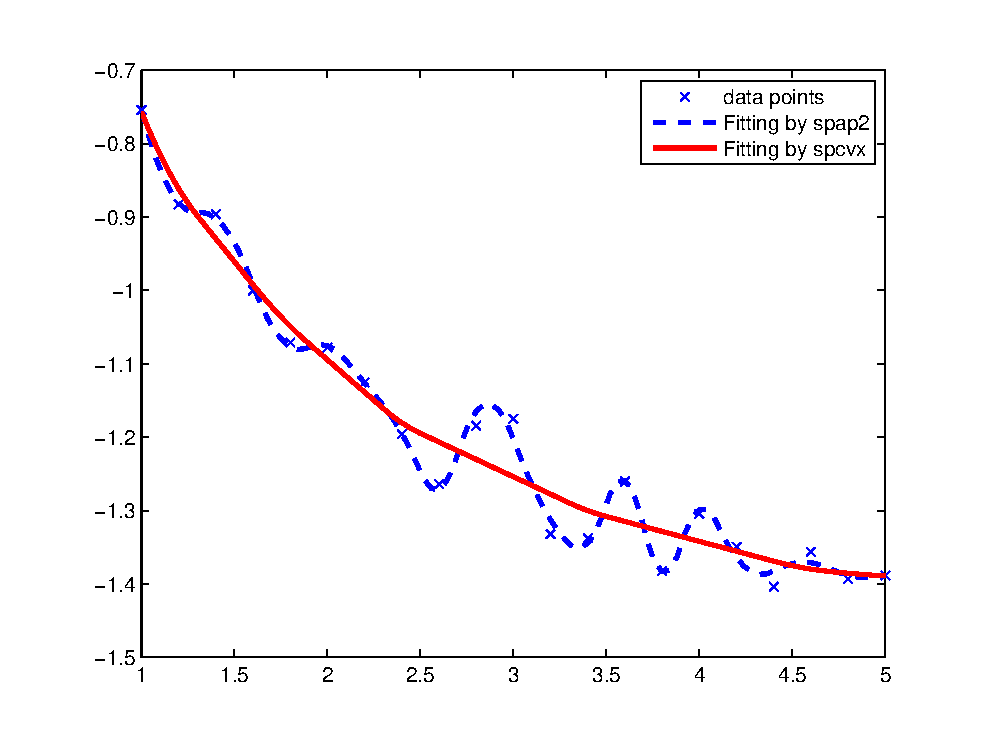
\includegraphics{cvxfit1d}}\\
    \caption{1-D Example.}\label{fig:cvxfit1d}
  \end{figure}


\Section{Tensor Product B-spline for Multivariate Data}
Multivariate data on rectangular grid can be fitted by tensor product B-splines.  
  \begin{figure}[ht]
    \centering
    \scalebox{0.55}{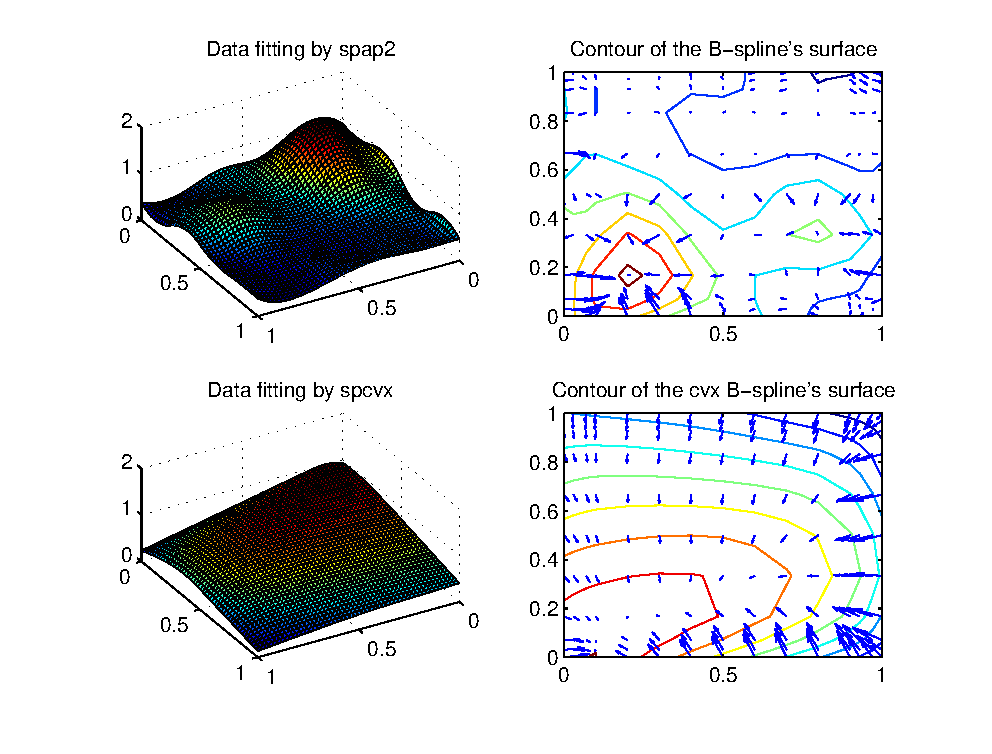
\includegraphics{cvxfit2d}}\\
    \caption{Bivariate case for gridded data}\label{fig:cvxfit2d}
  \end{figure}

  \begin{figure}[ht]
    \centering
    \scalebox{0.55}{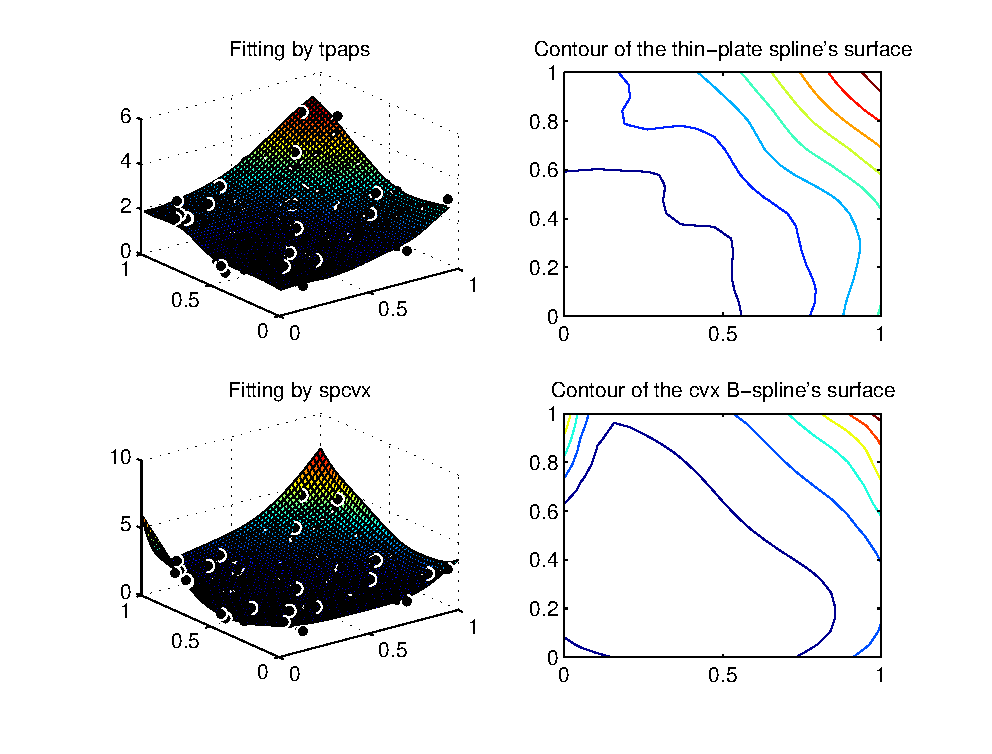
\includegraphics{cvxfitsd}}\\
    \caption{Bivariate case for scattered data}\label{fig:cvxfitsd}
  \end{figure}

  \begin{figure}[ht]
    \centering
    \scalebox{0.55}{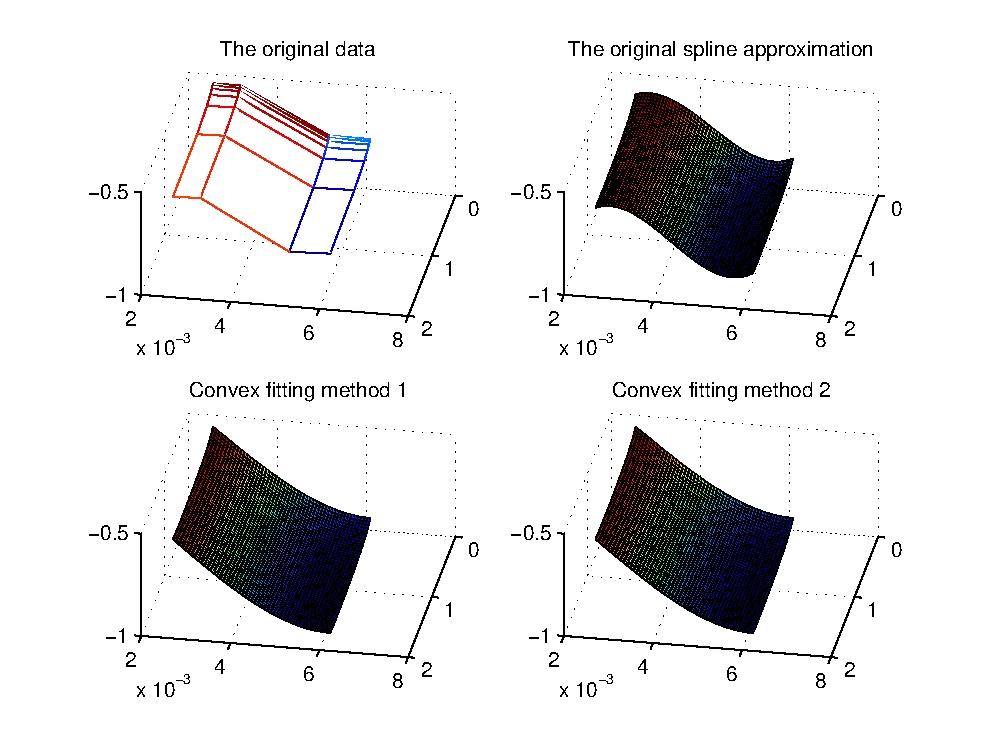
\includegraphics{cvxfitnd}}\\
    \caption{Multivariate case}\label{fig:cvxfitnd}
  \end{figure}

\Section{Summary}
  \begin{table*}
   \begin{center}
    \begin{tabular}{c|l|l|l|l|l}
      \hline
      & \small{CvxPWL} & \small{CvxFit} & \small{CvxSmth} & \small{SOS} & \small{B-spline} \\
      \hline
      \small{Convex formulation} & *      & ****   & ****    & ***** & *****    \\
      \hline
      \small{Smoothness}     & *  & ** & **** & ***** & ***** \\
      \hline
      \small{Convex preserve} & ***** & ** & **** & ***** & ***** \\
      \hline
      \small{Ease of fitting} & * & ***** & * & *** & ***** \\
      \hline
      \small{Ease of evaluation} & ***** & *** & *** & * & ***** \\
      \hline
      \small{Local support} & ***** & ***** & ***** & * & ***** \\
      \hline
    \end{tabular}
   \end{center}
  \end{table*}

\Section{Numerical Example}

\Section{Conclusions}

\bibliographystyle{latex8}
\bibliography{ref-cvxfit,refbibtex,ref-fitting}

\end{document}
